\documentclass[11pt]{scrartcl}
\usepackage{graphicx}
\usepackage{float}
\usepackage{amsmath}
 
\begin{document}
\title{Praktiukumsarbeit zum Praktikum Regelungstechnik}
\author{Christian Küllmer, Jonas Kallweidt, Leon Blum}
\date{\today{}, Kassel}
\maketitle
\newpage
%Inhaltsverzeichnis
\renewcommand{\contentsname}{Inhaltsverzeichnis}
\tableofcontents
\newpage

%Mathlab Aufgabe
\section{Rechnerteil Aufgaben aus Kapitel 9.3. des Praktikumsskrips}
In diesem Anteil geht es um die in Aufgabe 9.3a. Dieser bezeichnet das Aufstellen der Gleichungen aus den gegeben Gleichungen. Die Gleichungen sind gegen als Blockschaltbild gegeben. Diese werden jetzt übersetzt in Mathlab Simulink.

\begin{itemize}
\item Startwerte
Als Startwerte wurde gegeben:

\begin{align}
   	m &= 7\, kg
\end{align}
\begin{align}
   	l &= 1\, m
\end{align}
\begin{align}
   	g &= 9,81\, \frac{m}{s^2}
\end{align}
\begin{align}
   	c &= 1
\end{align}
\begin{align}
   	k &= 300  \\\\ T& = 0,1
\end{align}

	
	


\item Gegebenes Blockschaltbild:
\begin{figure}[H]
	\centering
	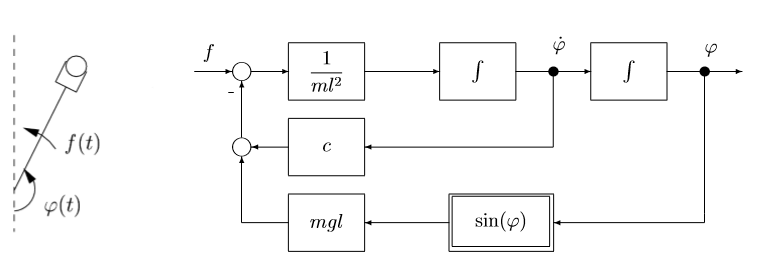
\includegraphics[width=0.6\textwidth]{Aufgabe9aMotorarm.png}
	\caption{Motorarmmodell als Blockschaltbild}
	\label{img:grafik-dummy}
\end{figure}
\begin{figure}[H]
	\centering
	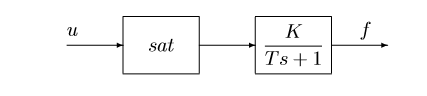
\includegraphics[width=0.6\textwidth]{Aufgabe9aStreckeMotor.png}
	\caption{Modell des Motors als Blockschaltbild}
	\label{img:grafik-dummy}
\end{figure}
\end{itemize}

%Version von Jonas und Christian vom 24.07.2019

\subsection{Aufgabe a) Gebautes Simulink Modell}
\begin{figure}[H]
	\centering
	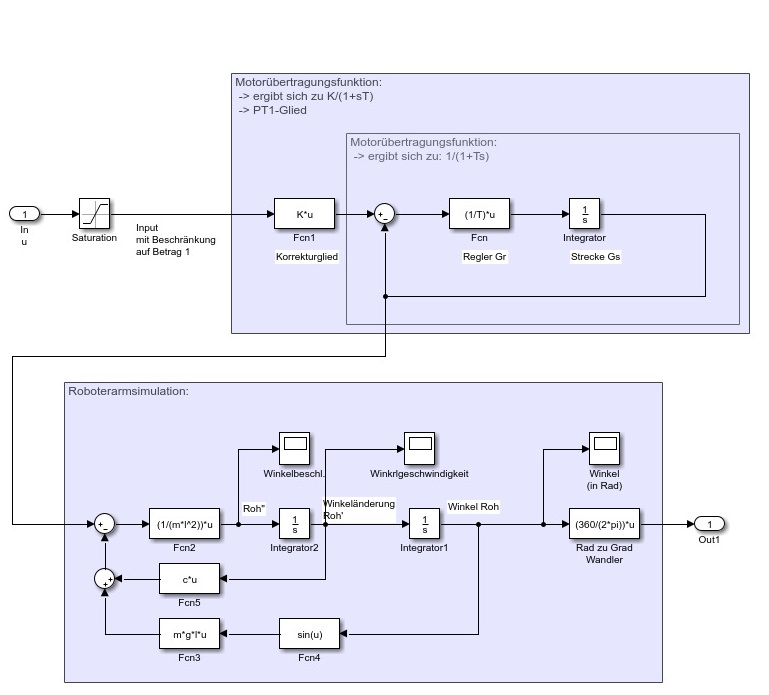
\includegraphics[width=0.7\textwidth]{SimulinkModell.jpeg}
	\caption{In Simulink gebautes Modell des Systems des Roboterarms}
	\label{img:grafik-dummy}
\end{figure}

%Version von Jonas und Christian vom 24.07.2019

\subsection{Aufgabe b)}
Das System wird simuliert und die Zustandsgrößen werden über einen Zeitverlauf dargestellt. Dabei entstehen folgende Diagramme:

\begin{figure}[H]
	\centering
	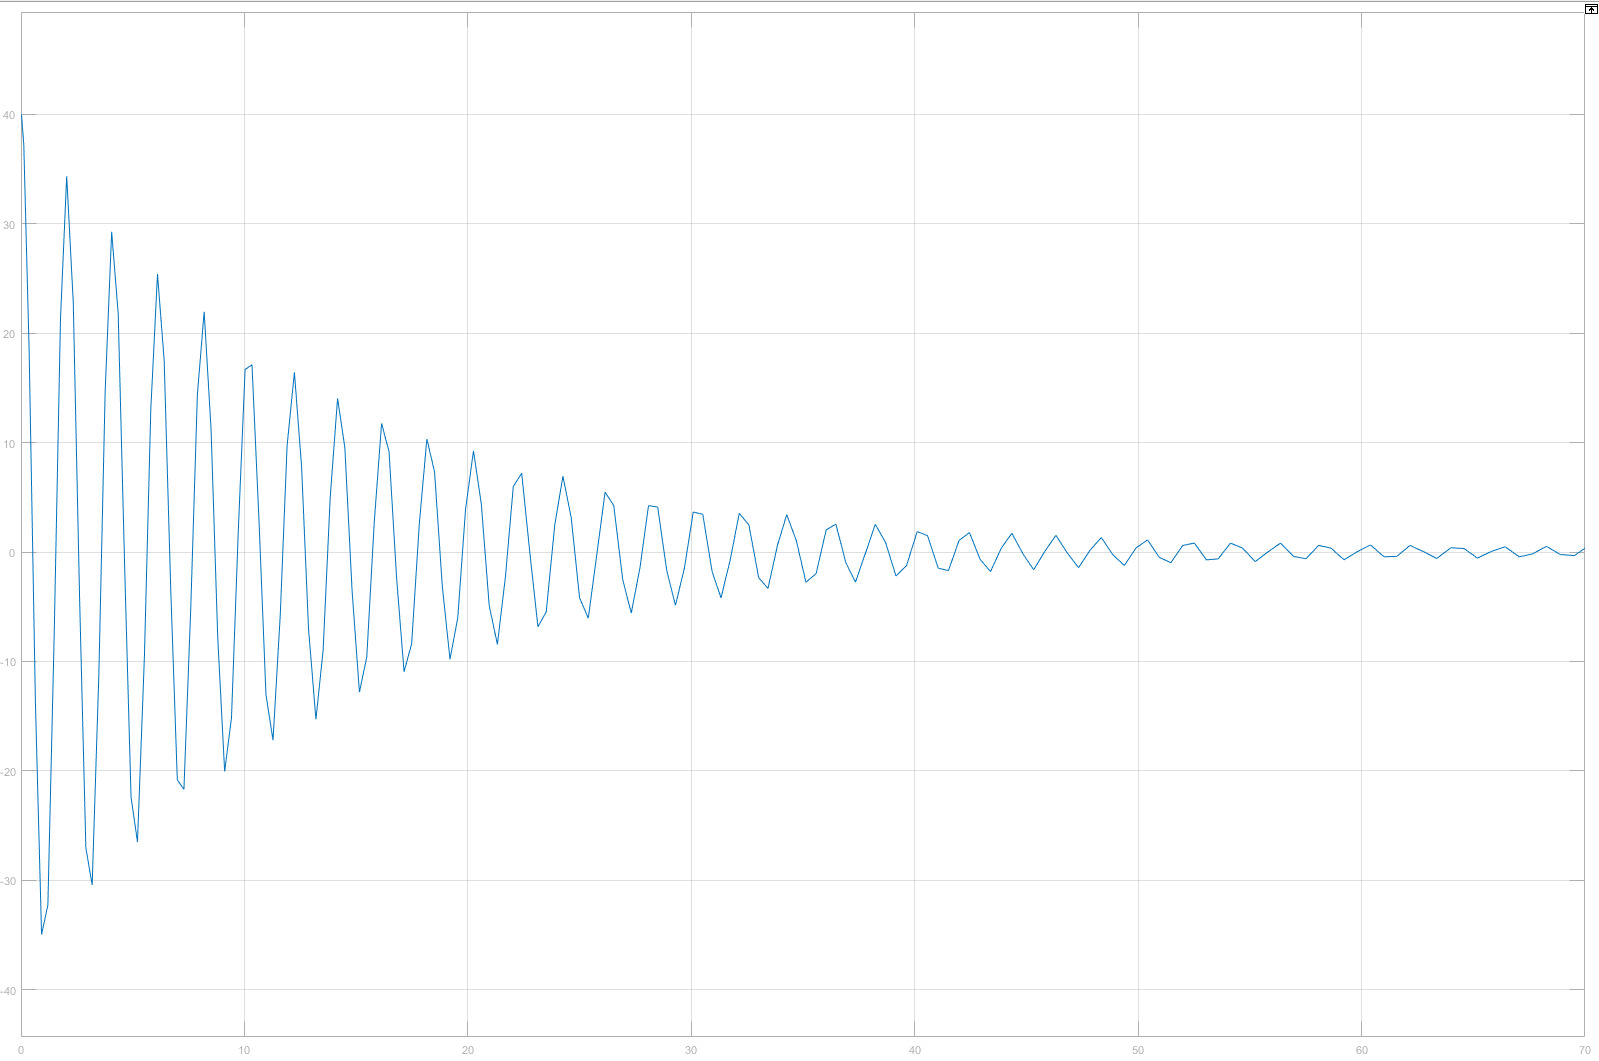
\includegraphics[width=1\textwidth]{WinkelanzeigeinGrad3b.jpeg}
	\caption{Darstellung des Winkels für eine anfängliche Auslenkung von 40 Grad. }
	\label{img:grafik-dummy}
\end{figure}
Aus dem Diagramm Figure 4 geht hervor, dass das System ein ungeregelt stabiles System darstellt, welches eine Ruhelage bei 0\,$^\circ$ annehmen kann, wenn vorher keine Auslenkung vorgenommen wurde. Hier geht die Auslenkung auf keinen stationären Endwert, da die Expotentialfunktion zur Beschreibung der Dämpfung niemals null wird. In einem Realen System wird hier aber wahrscheinlich ein Stillstand nach beliebig langer Wartezeit eintreten, wenn der Roboterarm die Haftreibung nicht mehr Überwinden kann und die Bewegung im Aperiodischen Grenzfall endet.

\subsection{Aufgabe c)}

%Präsensversuche
\section{Versuch Antrieb}

\section{Versuch Schwebekörper}

\section{Versuch Kran}

%Modell zum Einfügen eines Bildes
%\begin{figure}[H]
%	\centering
%	\includegraphics[width=0.8\textwidth]{}
%	\caption{Teamlogo: Team A}
%	\label{img:grafik-dummy}
%\end{figure}
Hallo
\end{document}